\documentclass[titlepage]{article}
\usepackage{pgfplots}

\begin{document}

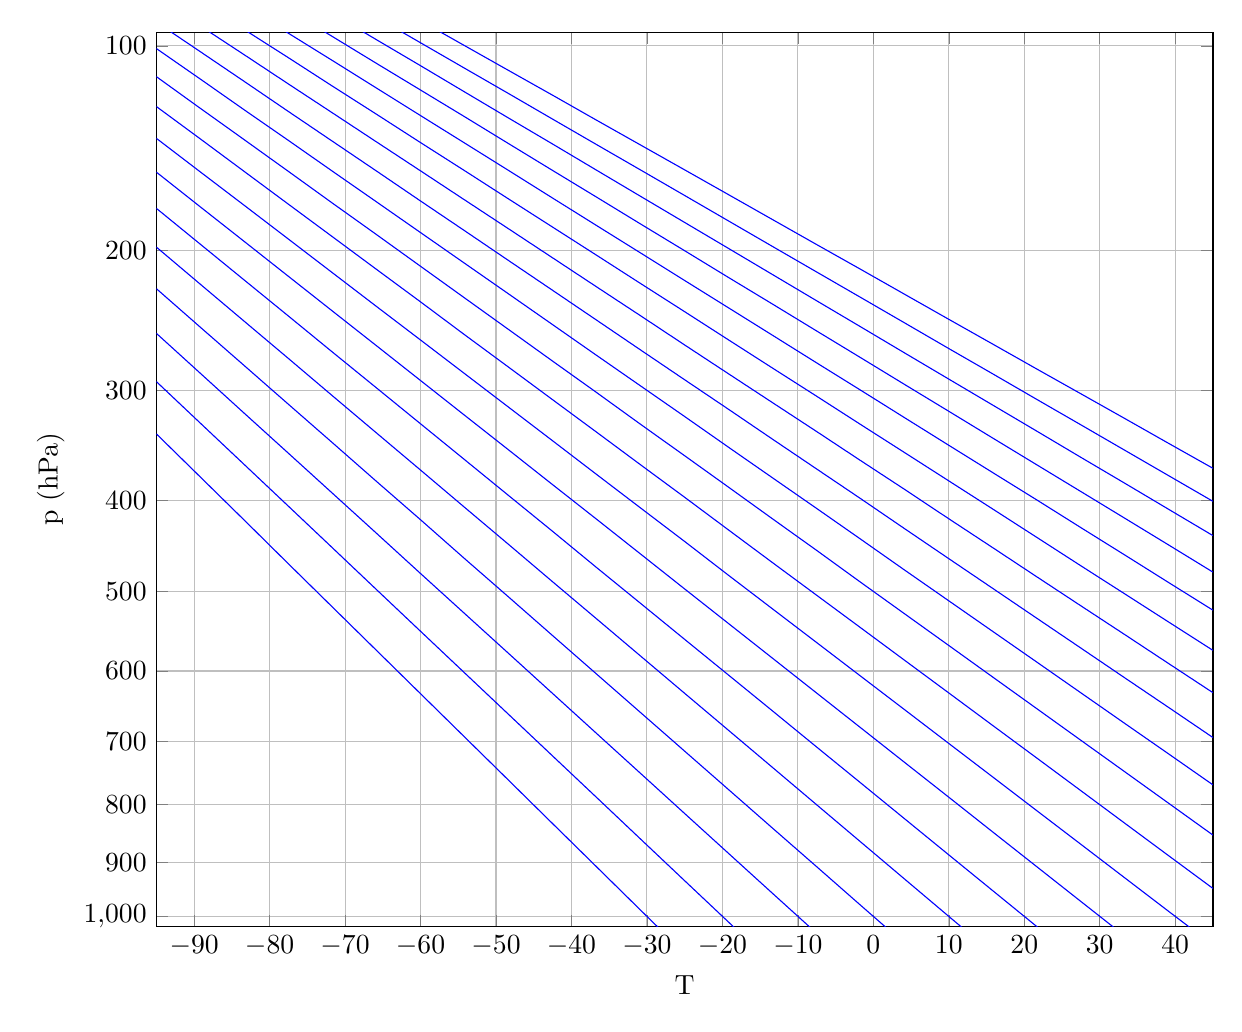
\begin{tikzpicture}
  \begin{axis}[
      xmin=-95,
      xmax=45,
      ymin=95,
      ymax=1020,
      y dir=reverse,
      ytick={100,200,...,1000},
      yticklabel style={/pgf/number format/.cd, precision=0, relative*=2},
      xlabel=T,
      ylabel=p (hPa),
      grid=both,
      width=15cm,
      y coord trafo/.code={\pgfmathparse{#1^0.286}},
      y coord inv trafo/.code={\pgfmathparse{#1^(1/0.286)}},
    ]
    \foreach \T in {-30,-20,..., 150} {
        \addplot [blue, domain=-95:45] {1000*((273.15+x)/(273.15+\T))^(1/0.286)};
      };
  \end{axis}
\end{tikzpicture}

\end{document}
